%!TEX root = ../thesis.tex
%Adding the above line, with the name of your base .tex file (in this case "thesis.tex") will allow you to compile the whole thesis even when working inside one of the chapter tex files

\chapter{Multi-wavelength Radio Continuum Emission Studies of \\ Dust-free Red Giants} \label{chap:6}

The vast increase in bandwidth coverage of the new VLA now allows possible detections of historically weak or undetectable red giants at multiple radio wavelengths. In this chapter, we present and analyze the most comprehensive set of multi-wavelength thermal radio continuum observations of two standard luminosity class III red giants, Arcturus ($\alpha$ Boo: K2 III) and Aldebaran ($\alpha$ Tau: K5 III), to date. We report the first detections at several wavelengths for each star including a detection at 10 cm (3.0 GHz: S band) for both stars and a 20 cm (1.5 GHz: L band) detection for $\alpha$ Boo. This is the first time single luminosity class III red giants have been detected at these continuum wavelengths. We compare our data with published semi-empirical atmospheric models based on UV data, and spectral indices are used to discuss the possible properties of the stellar atmospheres. Finally, we develop a simple analytical wind model for $\alpha$ Boo based on our new long wavelength flux measurements. This chapter is based on the main results of \cite{ogorman_2013}.

\section{Why Study Red Giants with the VLA?}\label{sec:6.1}
Although studies of wind-scattered UV and optical line profiles have provided clues to the mass-loss rates and radial distribution of the mean and turbulent velocity fields, the thermal structure remains poorly constrained. In the UV, the source function $S_{\nu}$, of electron collisionally excited emission lines is sensitive to electron temperature $T_{\rm{e}}$, (i.e., $S_{\nu} \propto e^{-h\nu /kT_{\rm{e}}}/\sqrt{T_{\rm{e}}}$). Therefore, a localized hot plasma component in a dynamic atmosphere can completely dominate the temporally and spatially averaged emission and hence not reflect the mean radial electron temperature distribution. At radio wavelengths however, the source function is thermal and is just the Rayleigh-Jeans tail of the Planck function, which is linear in electron temperature (i.e., $S_{\nu} = {2kT_{\rm{e}}\nu ^2 /c^2}$). This should give a more appropriate estimate of the mean radial electron temperature. It is this value that controls the atomic level populations and ionization of the mean plasma which is needed to quantify the implied thermal heating supplied to the  wind by the unknown driving source/sources, allowing constraints on potential mass-loss mechanisms to be derived.

In the cm-radio regime the radio opacity $ \kappa _{\lambda}$, strongly increases with wavelength (i.e., $ \kappa _{\lambda} \propto \lambda ^{2.1}$) and so the longer wavelengths sample the extended layers of a stars atmosphere, thus providing us with spatial information about the star's mass outflow region. The VLA is sensitive to over three orders of magnitude in continuum optical depth $\tau _{\lambda}$, ($\tau _{20 \ \rm{cm}}/\tau _{0.7 \ \rm{cm}} \approx 10^3$) and provides an area-averaged sweep through the wind acceleration zone of evolved late-type stars. The thermodynamic properties in this spatial region control the ionization in the far wind because the ionization balance, which also controls the cooling rates, becomes \textit{frozen-in} at large radii due to advection. Furthermore, it is these outer extended regions of the star's atmosphere that contribute to the commonly seen P Cygni line profiles in the UV. In these profiles the line-of-sight absorption caused by the star's wind is superimposed on the blueshifted scattered emission. Thus, centimeter radio continuum observations can provide a test of models based on these UV profiles. 

Despite the importance of radio continuum emission as a tool for studying cool evolved stellar outflows, red giants are feeble emitters at these wavelengths however, and previous observations have provided only a small number of modest signal-to-noise measurements slowly accumulated over three decades. As most of our VLA observations were carried out over just a few days, we have obtained a unique snapshot of the different stellar atmospheric layers sampled at different wavelengths, independent of any long-term variability. 

\section{Radio Maps}\label{sec:6.2}
Apart from $\alpha$ Boo at C band and $\alpha$ Tau at S band, detections were made in every sub-band for the 2011 data. For all other bands, the flux densities of the targets in both sub-bands were found to be the same within their uncertainties so we do not present separate values here. Instead we give the values from the radio maps produced by concatenating the two sub-bands. We present in Table \ref{tab:6.1} the target flux densities extracted from these concatenated radio maps. In each of these maps the flux density from the unresolved target source was calculated by, 1) taking the peak pixel value from the source, 2) manually integrating the flux density around the source, and 3) fitting an elliptical Gaussian model to the source and deriving the integrated flux density using the CASA \textit{imfit} task. Each of these values along with the image rms noise measured from adjacent background regions and fitting error produced by \textit{imfit} are given in Table \ref{tab:6.1} to indicate the quality of each radio map. Both sources are point sources at all frequencies so the peak flux value given in Table \ref{tab:6.1} will also be its total flux density value. For weak detections (i.e., $F_{\nu} \lesssim 5\sigma$) we avoid using the \textit{imfit} task to obtain a flux density estimate, as this may produce biased parameter estimates \citep{taylor_1999}. The flux density values used in the following Sections are the peak values listed in Table \ref{tab:6.1}. We assume absolute flux density scale systematic uncertainties of  3\% at all frequencies \citep{perley_2013}. In the following two sections we briefly discuss the properties of these maps for both targets which are shown in Figure \ref{fig6.2}.



\begin{figure}[htp]
\centering 
\mbox{
		  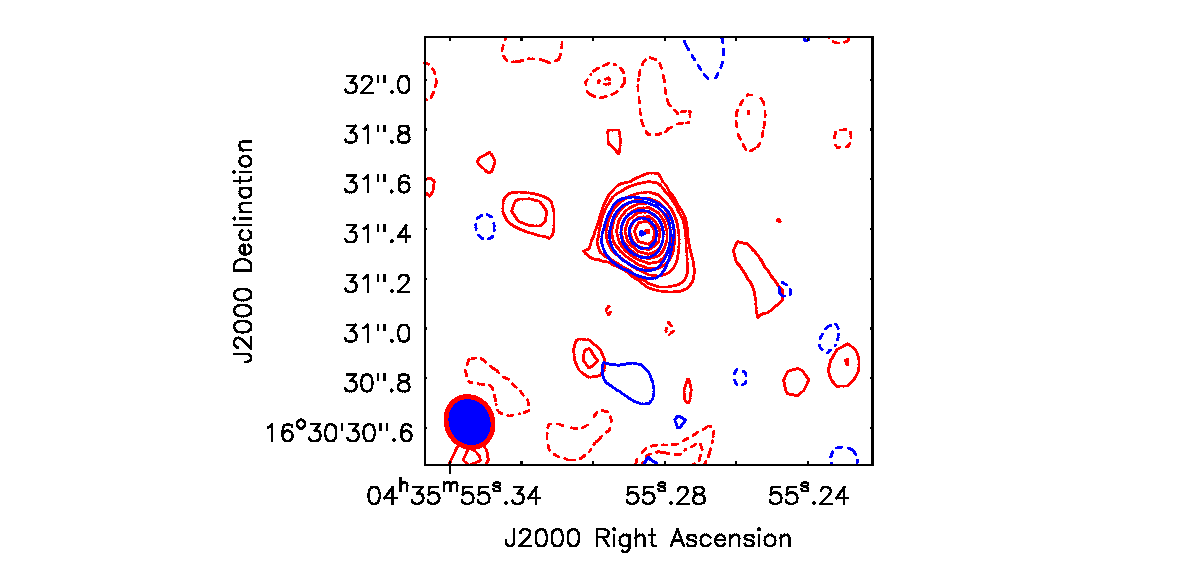
\includegraphics[trim=100pt 50pt 150pt 10pt,clip,width=7.5cm,height=6.0cm]{/home/eamon/thesis/thesis_template/6/atau_q_ka.ps}
          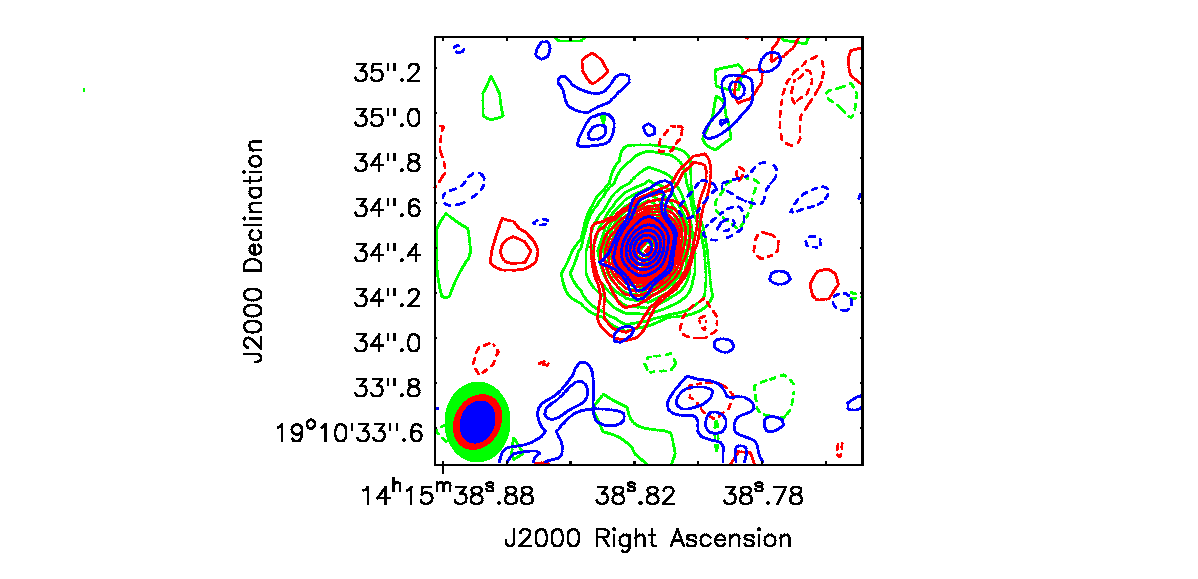
\includegraphics[trim=130pt 50pt 150pt 10pt,clip,width=7.5cm,height=6.0cm]{/home/eamon/thesis/thesis_template/6/aboo_q_ka_k.ps}
          }
\mbox{
          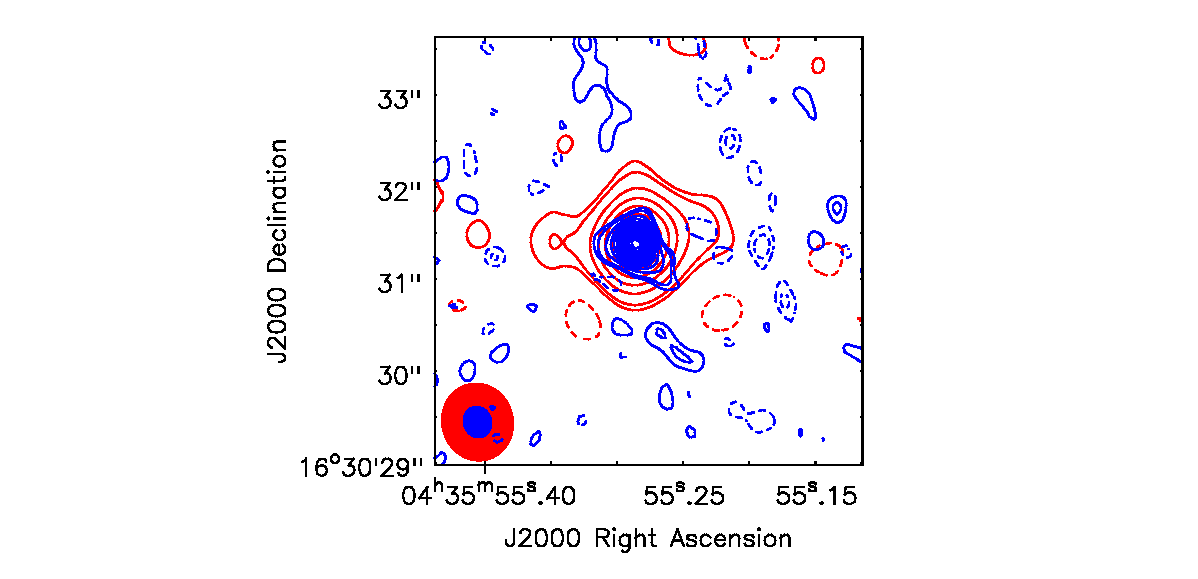
\includegraphics[trim=115pt 50pt 155pt 10pt,clip,width=7.5cm,height=5.8cm]{/home/eamon/thesis/thesis_template/6/atau_x_k.ps}
          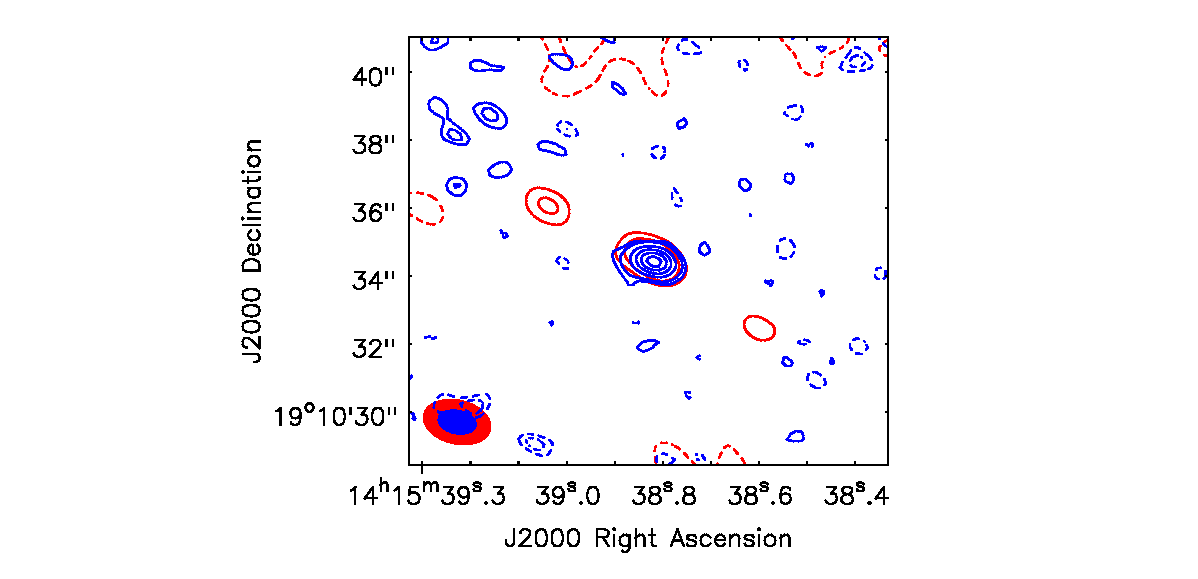
\includegraphics[trim=108pt 50pt 145pt 10pt,clip,width=7.3cm,height=5.8cm]{/home/eamon/thesis/thesis_template/6/aboo_c_x.ps}
          }
\mbox{
          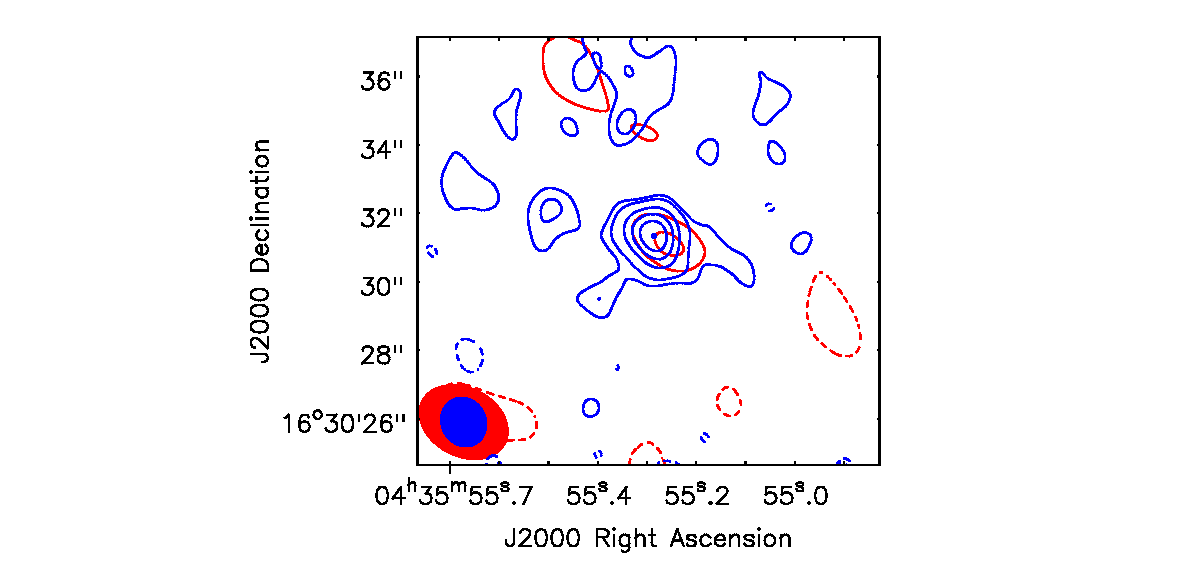
\includegraphics[trim=100pt 10pt 148pt 10pt,clip,width=7.5cm,height=6.4cm]{/home/eamon/thesis/thesis_template/6/atau_c_s.ps}
          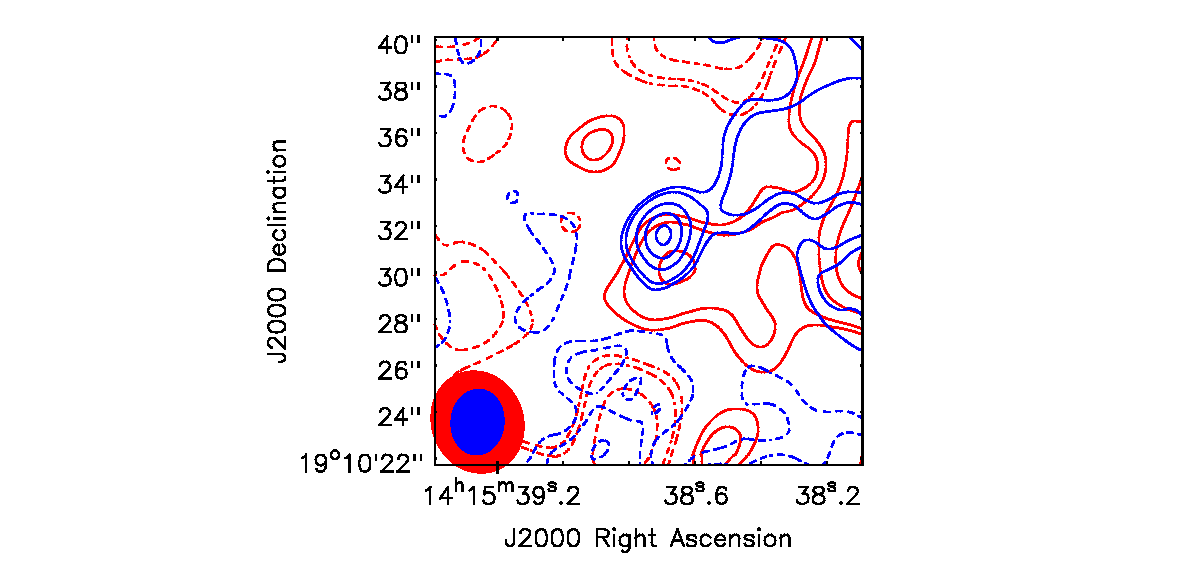
\includegraphics[trim=125pt 10pt 150pt 10pt,clip,width=7.5cm,height=6.4cm]{/home/eamon/thesis/thesis_template/6/aboo_l_s_ddt.ps}
          }
\caption[Final VLA multi-wavelength radio maps of $\alpha$ Boo and $\alpha$ Tau]{Final VLA multi-wavelength radio maps of $\alpha$ Tau and $\alpha$ Boo. \textit{Left column:} Q and Ka band (top), K and X band (middle), C and S band (bottom) maps of $\alpha$ Tau. \textit{Right column:} Q, Ka, and K band (top), X and C band (middle), S and L band (bottom) maps of $\alpha$ Boo. Contour levels are set at $(-6,-3,-2,+2,+3,+6,+9,....)\times \sigma$ where $\sigma$ is the rms noise of each radio map. For $\alpha$ Boo, artifacts from the dirty beam can be seen in the Q band map, while artifacts caused by the serendipitous strong source in the S and L band maps are also present.}
\label{fig6.2}
\end{figure}

\afterpage{\begin{landscape}
\begin{table}[!hb]
\begin{center}
\caption[VLA Flux Densities of $\alpha$ Boo and $\alpha$ Tau]
{VLA Flux Densities of $\alpha$ Boo and $\alpha$ Tau.}
\begin{tabular}{ccccccccc}
\hline
\hline
Star & Band & $\nu ^{\rm{a}}$ & $\lambda$ & Peak $F_{\nu}$ & Integrated  &\textit{Imfit} Integrated & Image rms &\textit{Imfit} Fitting \\
 &  & (GHz) & (cm) & (mJy beam$^{-1}$) & $F_{\nu}$ (mJy)& $F_{\nu}$ (\rm{mJy})&(mJy beam$^{-1}$)&Error (mJy)\\
\hline
\rule{0pt}{2.5ex}$\alpha$ Boo  &Q  &43.28&0.7 &5.94 & 6.09 & 6.42 & 0.30 &  0.26\\
&Ka &33.56&0.9& 4.16 & 4.32 & 4.49 & 0.08 & 0.09 \\
&K  &22.46&1.3& 1.83 & 1.78 & 1.81 & 0.04 & 0.05 \\
&X  &8.46&3.5 & 0.51 & 0.51 & 0.53 & 0.03 & 0.02 \\
&C  &4.90&6.1 & 0.21 & 0.14 & 0.16 & 0.04 & 0.01 \\
&S  &3.15&9.5 & 0.15 & 0.14 & -     & 0.03 & -     \\
&S  &2.87&10.4 & 0.13 & 0.12 & 0.12 & 0.01 & 0.02\\
&L  &1.63&18.4 & 0.07 & 0.07 & -     & 0.01 & -    \\
\hline
\rule{0pt}{2.5ex}$\alpha$ Tau &Q  &43.28 & 0.7&3.67& 3.73 & 4.08 &  0.26& 0.18	\\
&Ka &33.56 & 0.9&2.19& 1.96 & 2.13 &  0.09& 0.07 \\
&K  &22.46 &1.3& 1.86& 1.88 & 2.07 &  0.04& 0.08 \\
&X  &8.46  & 3.5&0.30& 0.29 & 0.28 &  0.01& 0.02 \\
&C  &4.96  & 6.0&0.15& 0.17 & 0.18 &  0.01& 0.01 \\
&S  &3.15  & 9.5&0.06& 0.04 & - &  0.02 & -\\
\hline
\end{tabular}
\label{tab:6.1}
\begin{minipage}{19.cm}
$^{\rm{a}}${\footnotesize Frequency of the final image produced using the multi-frequency synthesis imaging mode within CASA's \textit{clean} task.}
\end{minipage}
\end{center}
\end{table}
\end{landscape}}

\subsection{$\alpha$ Boo Maps}\label{sec:6.2.1}
High S/N detections ($>$19$\sigma$) of $\alpha$ Boo were made at 22.5, 33.6, and 43.3 GHz. Some residuals of the dirty beam remained in the CLEANed maps due to the paucity of uv-coverage in these short high frequency observations (see Figure \ref{fig6.2}, top right panel). At the lower frequencies, it was necessary to image confusing sources, notably a strong radio source located $186\arcsec$ north-west of $\alpha$ Boo. This non-thermal source was reported by \cite{drake_1983} and their flux density of 25 mJy at 4.9 GHz is in close agreement with our measurement of 23.2 mJy at the same frequency. We find the source to have a spectral index $\alpha$ ($F_{\nu} \propto \nu ^{\alpha}$) of -1.4 between 8.5 and 1.6 GHz; its flux density reaches 80.3 mJy at 1.6 GHz.

We detected $\alpha$ Boo at 6$\sigma$ in the lower frequency sub-band of C band, at 4.9 GHz. The noise was slightly higher and the images were poorer quality in the C band higher frequency sub-band, with artifacts exceeding $\pm$200 $\mu$Jy, and we cannot report a detection in this sub-band, so values given in Table \ref{tab:6.1} are taken from the lower frequency sub-band only. We obtain good detections ($>$5$\sigma$) of the star for both epochs at $\sim 3$ GHz (S band) and the peak flux densities agree within their uncertainties. We can therefore safely assume that the 1.5 GHz (L band) flux density has not changed significantly over that period either, and so can safely be included in any analysis. The map at L band was highly contaminated by the sidelobes of the strong source north-west of $\alpha$ Boo but the star is still detected at the $5\sigma$ level. There is a slight positional offset of $1\arcsec$ between the position of the peak flux density at 1.5 and at 3.0 GHz for the 2012 data, which were taken within 1 day of each other. However, the position uncertainties due to noise and phase uncertainties between the directions of the phase reference source and the target are at least $1\arcsec$, and so we feel that it is highly likely that both detections are of $\alpha$ Boo.

\subsection{$\alpha$ Tau Maps}\label{sec:6.2.2}
The final deconvolved radio maps of $\alpha$ Tau were of excellent quality with the rms noise reaching the predicted noise levels in many cases. The target field at all frequencies was free from strong serendipitous radio sources and thus the final images were free of the sidelobe contamination that were present in the low frequency $\alpha$ Boo images. $\alpha$ Tau was the only source in the high frequency maps while the brightest source in the low frequency maps was located $106\arcsec$ north north-east of $\alpha$ Tau and had flux densities of 0.85, 1.35, and 1.7 mJy at 8.5, 5.0, and 3.5 GHz, respectively. Detections of high significance ($>$14$\sigma$) were made at all frequencies between 5.0 and 43.3 GHz for $\alpha$ Tau. Due to the limited number of S band receivers available at the time, a full 2.5 hr track was dedicated to $\alpha$ Tau at 3.1 GHz in order to achieve the required sensitivity to give a possible detection. We report a tentative $3\sigma$ detection of $\alpha$ Tau at 3.1 GHz when we take its peak pixel value as its total flux density.

\section{Results Versus Previous Observations}\label{sec:6.4}
Prior to and during the early operation of the ``old'' VLA, a small number of single dish radio observations, such as those from the Arecibo \citep{boice_1981} and Parkes \citep{slee_1989} radio telescopes, reported the detection of flares from single red giants. These transient radio events have never been re-observed however, even with more sensitive interferometers, suggesting that such detections were spurious (e.g., \citealt{beasley_1992}). The first definitive detection of thermal free-free emission from a luminosity class III single red giant at centimeter wavelengths was of $\alpha$ Boo at 6 cm \citep{drake_1983,drake_1986}. Since then there has been a modest number of centimeter and millimeter observations of this star. In Table \ref{tab:6.4.1} we list the majority of these observations and plot their flux densities as a function of frequency in Figure \ref{fig6.4.1} (red diamonds). In comparison to other single red giants, $\alpha$ Boo had been relatively well observed at radio continuum wavelengths before this study, including detections in four VLA bands (i.e., Q, K, Ku, and C). No Ku band receivers were available during the commissioning phase of the VLA in early 2011 so we can compare three of our detections with previous ones.

\begin{table}[!hbt]
\begin{center}
\caption[Compilation of Previous Radio Observations ($\nu \le 250$ GHz)]
{Compilation of Previous Radio Observations ($\nu \le 250$ GHz).}
\begin{tabular}{cccccc}
\hline
\hline
\rule{0pt}{2.5ex}Source & $\nu$ (GHz) & Date &  $F_{\nu}$ (mJy) & S/N & Reference\\
\hline
$\alpha$ Boo &4.9  & 1983 Jan 21 & 0.39 & 3.0 & 1 \\
&4.9  & 1983 May 20 & 0.26 & 3.3& 1 \\
&4.9  & 1983 Dec 26 & $\le$0.18$(3\sigma)$&- & 1 \\
&4.9  & 1984 Mar 17 & 0.24  & 4.8& 1 \\
&15.0 & 1984 Nov 6 & 0.68 & 7.6& 1 \\
&22.5  & 1999 Jan 06  &1.7& 8.5& 2 \\
&43.3  & 1999 Jan 06 & 3.3& 8.3& 2 \\
&43.3  & 2004 Jan 25 & 3.34& 41.8& 2 \\
&86.0  & 1985 Nov  & 21.4& 3.0& 3 \\
&108.4  & 1997 Nov - 2000 Jun & 20.1 &29.1 & 4 \\
&217.8 & 1997 Nov - 2000 Jun  & 83.5 &48.8 & 4 \\
&250.0  & 1986 Dec - 1989 Mar  & 78.0 & 9.8& 5 \\
\hline
\rule{0pt}{3ex}    $\alpha$ Tau	&4.9  & 1983 Jan 21 & $\le$0.27$(3\sigma)$&-& 1 \\
&4.9  & 1984 Nov 6 & $\le$0.22$(3\sigma)$&-& 1 \\
&5.0  & 1997 Sep 27 & $\le$0.07$(3\sigma)$	&-& 6 \\
&8.5  & 1997 Sep 27 & 0.28 	&9.3	& 6 \\
&14.9 & 1997 Sep 27 & 0.95 	&11.9	& 6 \\
&15.0 & 1984 Nov 6 & 0.60 	&6.0	& 1 \\
&108.4  & 1997 Nov - 2000 Dec &  14.0  & 9.6& 4 \\
&217.8 & 1999 Sep - 2000 Dec  & 25.8 & 4.6& 4 \\
&250.0  & 1986 Dec - 1987 Jan & 51.0 & 8.5& 5 \\
\hline
\end{tabular}
\label{tab:6.4.1}
\begin{minipage}{13.5cm}
\rule{0pt}{3ex} References.-(1) \cite{drake_1986}; (2) \cite{dehaes_2011}; (3) \cite{altenhoff_1986}; (4) \cite{cohen_2005}; (5) \cite{altenhoff_1994}; (6) \cite{wood_2007}. 
\end{minipage}
\end{center}
\end{table}

Previous detections of $\alpha$ Boo at 6 cm ranged from a 3$\sigma$ upper limit of 0.18 mJy to a 3$\sigma$ detection at 0.39 mJy. Our 6 cm value agrees to within $\sim$10$\%$ of the highest S/N (5$\sigma$) value of \cite{drake_1986}. There is no significant difference between our 1.3 cm value and that of \cite{dehaes_2011}. There is however a notable difference in flux density values at 0.7 cm  where \cite{dehaes_2011} report values that are lower than ours by over 40\%. Although we do not rule out such a level of chromospheric radio variability, it is not expected based on the small level of UV variability observed from such supposedly inactive stars \citep{harper_2013}. Another possibility for the difference in values is that the longer cycle time used by \cite{dehaes_2011}, which was over double our value, may lead to larger phase errors and thus lower final flux density values. Future high frequency VLA observations of $\alpha$ Boo will clarify this discrepancy at 0.7 cm but past detections at longer wavelengths appear to be in good agreement with our data.

\afterpage{\begin{landscape}
\begin{figure*}[!hb]
\centering 
         \includegraphics[trim=5pt 0pt 28pt 0pt,clip, scale=0.70, angle=90]{/home/eamon/thesis/thesis_template/6/aboo_summary.ps}
\caption[Spectral energy distribution of $\alpha$ Boo]{Spectral energy distribution of $\alpha$ Boo for 1 GHz $\leq \nu \leq$ 1 THz. Our new multi-frequency VLA observations which were mainly acquired over a few days in February 2011 are the blue circles and disagree with the existing chromospheric and wind models of \cite{drake_1985}. The overlap between the two models is represented by the green shaded area. The red diamonds are previous observations which were acquired sporadically over the last three decades with the `old' VLA, IRAM and BIMA. The black dashed line is the expected radio emission from the Drake model which undergoes rapid wind cooling beyond $\sim$2.3 $R_{\star}$ (see Section \ref{sec:6.6} and \ref{sec:6.7}).}
\label{fig6.4.1}
\end{figure*}
\end{landscape}}

\afterpage{\begin{landscape}
\begin{figure*}
\centering 
         \includegraphics[trim=5pt 0pt 28pt 0pt,clip, scale=0.70, angle=90]{/home/eamon/thesis/thesis_template/6/atau_summary.ps}
\caption[Spectral energy distribution of $\alpha$ Tau]{Spectral energy distribution of $\alpha$ Tau for 1 GHz $\leq \nu \leq$ 1 THz. Our new multi-frequency VLA observations of $\alpha$ Tau (blue circles) were acquired in just two days in February 2011. The red diamonds are the previous radio observations of the star which were acquired over many years (see Table \ref{tab:6.1}). The green line is the expected radio emission from the existing hybrid chromosphere and wind model, while the dashed  green line is the expected radio emission from a theoretical Alfv\'en wave driven model atmosphere.}
\label{fig6.4.2}
\end{figure*}
\end{landscape}}

In Figure \ref{fig6.4.2} we plot the previous  radio measurements of $\alpha$ Tau at all frequencies below 250 GHz (i.e. $> 0.12$ cm). Prior to this study, $\alpha$ Tau had only been detected at two VLA bands (i.e., X and Ku) and had never been detected at wavelengths longer than 3 cm due to its relatively low mass-loss rate. Our lack of a Ku band measurement means that we can only compare the previous 3 cm detection reported in \cite{wood_2007} to ours. We find that there is no significant difference between the two. Interestingly, \cite{wood_2007} report a non-detection of $\alpha$ Tau at 6 cm and placed a 3$\sigma$ upper limit of 0.07 mJy on its emission. In stark contrast to this, we were able to detect the star at 6 cm with a flux density over two times greater than this value. This hint of variability at long wavelengths would be consistent with the predictions of the broadband nonlinear Alfv\'{e}n wave model of \cite{airapetian_2010} but can again only be confirmed with future high S/N observations.

\section{Results Versus Existing Models}\label{sec:6.5}
One of the most important diagnostic features indicating mass outflows in late-type evolved stars are the blue shifted absorption components present in the \ion{Ca}{ii} H and K and Mg\,\textsc{ii} h and k resonance lines\footnote{Examples of these features are shown in Figures \ref{fig:1.2.2} and \ref{fig:3.4.1}.}. Figure \ref{fig6.5.1} shows one of the two chromosphere and wind models of $\alpha$ Boo \cite[`model A']{drake_1985} which is based on the Mg\,\textsc{ii} k 2796 $\rm{\AA}$ emission line observed with the International Ultraviolet Explorer. The line was modeled by solving the radiative transfer equation in a spherical co-moving frame and the effects of partial redistribution \citep[e.g.,][]{drake_1983b} were taken into account. Both of Drake’s atmospheric models
are semi-empirical and contain no assumptions about the wind driving mechanism. They contain the photospheric model of \cite{ayres_1975}, predict the wind to reach a terminal velocity of 35 - 40 km s${}^{-1}$ by 2 $R _{\star}$, and reach a maximum microturbulence of 5 km s$^{-1}$. They contain a broad temperature plateau with $T_{\rm{e}}$ $\approx$ 8,000 K between 1.2 and $\sim$20 $R _{\star}$ with a cooler region farther out, and hydrogen is 50\% ionized throughout. We compute the radio spectrum from these models assuming spherical 1-D geometry \citep{harper_1994} with the free-free Gaunt factors from \cite{hummer_1988}. The radiative transfer equation is solved using the Feautrier technique \citep{mihalas_1978} and the boundary condition is determined by ensuring the atmosphere is optically thick at the deepest layers. \cite{drake_1985} predicts that their atmospheric model would produce a flux density value of 0.4 mJy at 6 cm and encouragingly, our radio spectrum reproduces this value. Departures from spherical symmetry are to be expected in magnetic stellar atmospheres. For example, $\alpha$ Boo has an inclination axis of 58$^{\circ} \pm$25$^{\circ}$ \citep{gray_2006} and a global magnetic dipole could cause density variations between the equator and the polar regions. Despite this fact, the study of a  spherically symmetric atmosphere forms the basis of understanding the more complex environments in real stellar atmospheres.

\begin{figure}[t!]
\centering 
          \includegraphics[trim=0pt 0pt 0pt 0pt,clip,width=11.0cm, angle=90]{/home/eamon/thesis/thesis_template/6/drake_vs_mc_robinson.ps}
\caption[1-D semi-empirical model atmospheres for $\alpha$ Boo and $\alpha$ Tau]{1-D semi-empirical model atmospheres for $\alpha$ Boo and $\alpha$ Tau. The dashed red line is the model atmosphere for $\alpha$ Boo \citep{drake_1985} while the solid black line is the model atmosphere of $\alpha$ Tau which consists of the chromosphere and transition region model of \cite{mcmurry_1999} and the wind model of \cite{robinson_1998}.}
\label{fig6.5.1}
\end{figure}

Figure \ref{fig6.4.1} shows the resulting predicted radio spectrum between 1 GHz and 1 THz for $\alpha$ Boo from these chromosphere and wind models (green line). At high frequencies the radio spectra produced by these models have a blackbody-like slope (i.e., $\sim \nu ^{2}$) as a result of the small ion density scale heights close to the star where the temperature is changing slowly. At low frequencies however, where the Drake models predict the wind to have constant velocity, ionization fraction, and temperature, the slopes approaches the well known $\sim\nu ^{0.6}$ limit \citep{wright_1975,olnon_1975,panagia_1975}. The paucity and, in some cases low S/N, of previous observations made it difficult to discern the validity of this model prior to our multi-frequency study of $\alpha$ Boo. Our new data reveal significant deviations from the semi-empirical model at both low and high frequencies (in this case below $\sim 8$ GHz and above $\sim 25$ GHz). At high frequencies our VLA data indicates a flux excess which is in agreement with previous mm-observations. This may be due to larger chromospheric ion densities or to the possible presence of transition region plasma not accounted for in the Drake model. The discrepancy at low frequencies may be due to a lower ionization fraction in the wind, or a lower mass-loss rate than that used in the Drake model and this will be discussed further in Section \ref{sec:6.7}.

In Figure \ref{fig6.4.2} we plot the expected radio spectrum of $\alpha$ Tau based on the semi-empirical 1-D chromosphere and transition region model of \cite{mcmurry_1999} embedded in the 1-D wind model of \cite{robinson_1998}. The semi-empirical McMurry model was created by using the radiative transfer code MULTI \citep{carlsson_1986} to reproduce the fluxes of collisionally excited C\,\textsc{i}, C\,\textsc{ii}, Si\,\textsc{iii}, Mg\,\textsc{ii}, and C\,\textsc{iv} lines in a plane-parallel, hydrostatic, one-component atmosphere. It contains the photospheric model of \cite{johnson_1973} and reaches a maximum temperature of 10$^{5}$ K at 1.2 $R_{\star}$. As it does not contain a wind outflow, we use Robinson et al.'s wind characteristics beyond 1.2 $R_{\star}$ to describe the outflow velocity. In this wind model, the wind reaches $\sim$80\% of its terminal value of 30 km s$^{-1}$ by 3 $R_{\star}$. The Robinson et al. wind characteristics are based on matching the Fe\,\textsc{ii} 2755 $\rm{\AA}$ line and the O\,\textsc{i} triplet near 1304 $\rm{\AA}$ with a simplified wind model using the SEI computer code \citep{lamers_1987}. We assume the wind to have a constant temperature of 10,000 K and have a constant ionization fraction of $x_{e} = 0.6$ throughout, based on the ionization fraction at the corresponding temperature in the McMurry model. This idealized \textit{hybrid} model atmosphere for $\alpha$ Tau is plotted in Figure \ref{fig6.5.1}.

The radio flux densities at high frequencies (i.e., $\nu >$ 30 GHz) are overestimated by the combination of both atmospheric models, although this approach does well in reproducing the VLA flux densities below 30 GHz. The VLA, Institut de Radioastronomie Millim\'{e}trique (IRAM) 30 m-telescope and Berkeley Illinois Maryland Association (BIMA) continuum flux densities confirm that this model predicts a flux excess at even higher frequencies. One possible explanation for this is that the inner atmosphere contains extensive amounts of cooler gas than that predicted by the 1-D static chromospheric model of McMurry. This scenario agrees with the findings of \cite{wiedemann_1994} who conclude that cool regions exist close to the stellar surface with large ($> 99 \%$) filling factors i.e., a thermally bifurcated CO-mosphere \citep{ayres_1996}. The wind, which we have overlain on top of the McMurry chromosphere and transition region, is found to be optically thin at nearly all VLA wavelengths, and only contributes a very small flux density at the longest wavelengths. As our model matches the data reasonably well below 30 GHz we conclude that $\alpha$ Tau's wind is optically thin and the VLA radio emission at all wavelengths emanates from the inner atmosphere. 

We also include the predicted radio spectrum from the theoretical Alfv\'{e}n wave-driven outflow model for $\alpha$ Tau \citep{krogulec_1989} in Figure \ref{fig6.4.2} to demonstrate how radio observations can empirically challenge theoretical models. This model has a fully-ionized outflow inside 10 $R_{\star}$, and has a mass-loss rate of  6.3 $\times$ 10$^{-9}$ $M_{\odot}$ yr$^{-1}$, more than two orders of magnitude higher than the more recent estimate given in Table \ref{tab:6.1}. As the radio opacity is proportional to $n _{\rm{e}} n _{\rm{ion}}$, where $n_{\rm{e}}$ and $n_{\rm{ion}}$ are the electron and ion number densities respectively, this model greatly overestimates the actual radio flux density at all VLA wavelengths. The linear Alfv\'{e}n wave models for $\alpha$ Boo \citep{krogulec_1988} also assume full ionization and have higher mass-loss rates than the value given in Table \ref{tab:6.1}, predicting higher flux densities than observed. The lack of agreement between the Alfv\'en wave-driven wind models of \cite{krogulec_1988,krogulec_1989} and our observed radio fluxes may not necessarily be due to an incorrect  wind driving mechanism and instead may be due to the simplifications and  uncertainties in these models, such as wind densities, magnetic field strengths, damping lengths, and flow geometries close to the star. For example, the mass-loss rate is very sensitive to the radial surface magnetic field strength (i.e., $\dot{M} \propto B^4$) in these Alfv\'en wave models \citep{holzer_1983} so a small uncertainty in the magnetic field strength can lead to a large uncertainty in the mass-loss rate. Relaxing some of these simplifications such as purely radial flows or non-assumption of the WKB approximation \citep{charbonneau_1995} may also also lead to better agreement with our radio data.

\section{Spectral Indices}
\label{sec:6.6}
Long wavelength radio emission from non-dusty K spectral-type red giants is due to thermal free-free emission in their partially ionized winds while shorter wavelength radio emission emanates from the near static and more ionized lower atmospheric layers. The radio flux density-frequency relationship for these stars is usually found to be intermediate between that expected from the isothermal stellar disk emission, where $\alpha$ follows the Rayleigh-Jeans tail of the Planck function (i.e., $\alpha = +2$), and that from an optically thin plasma (i.e., $\alpha = -0.1$). We have shown in Chapter \ref{chap:1} that the expected radio spectrum from a spherically symmetric isothermal outflow with a constant velocity and ionization fraction varies as $\nu ^{0.6}$ \citep{wright_1975,olnon_1975,panagia_1975}. In reality however, thermal gradients will exist in the wind when the heating mechanisms become insufficient to counteract adiabatic and line cooling, so one would expect a temperature decrease in the wind at some point. Also, if the radio emission emanates from the wind acceleration zone then the electron density will not follow $n_{e} \propto r^{-2}$. 

We therefore relax some of the constant property wind model assumptions and assume that the electron density and temperature vary as a function of distance from the star $r$, and have the power-law form $n_{e} \propto r^{-p}$ and $T_{e} \propto r^{-n}$, respectively \citep[e.g.,][]{seaquist_1987}. Finding the spectral index for an outflow with these conditions is non-trivial, so we highlight the main steps required to do so here. We assume the same geometry and notation used for the constant property wind model in section \ref{sec:1.8.4} of Chapter \ref{chap:1}, and start by calculating the optical depth along a ray at position $z$ with an impact parameter $b$ through the atmosphere
\begin{equation}
\tau_{\nu}(b,z) =\frac{0.212Z^2n^2_{0}r_{0}^{2p-1.35n}}{\nu^{2.1}T_{0}^{1.35}}\int ^{z}_{-\infty} \frac{dz}{(b^2 + z^2)^{(2p - 1.35n)/2}} \equiv \int ^{z}_{-\infty} \frac{Cdz}{(b^2 + z^2)^{(2p - 1.35n)/2}},
\label{eq:eq6.6.1}
\end{equation}
where $T_{0}$ and $n_{0}$ are the gas temperature and density, respectively, at the base of the wind, $r_{0}$, and $C$ is a constant representing everything outside of the first integral. We have also assumed that the electron density is the same as the ion density throughout. 

The total flux density is found by integrating along the entire ray and over the entire sky
\begin{equation}
F_{\nu} = \frac{2\pi}{d^2}\int ^{\infty}_{z=-\infty}\int ^{\infty}_{b=0} B_{\nu}(z,b)\,\mathrm{exp}\left[-\tau_{\nu}(b,z)\right]b\,db\,dz,
\label{eq:eq6.6.4}
\end{equation}
and so we can now substitute in the Rayleigh Jeans function for $B_{\nu}$ (remembering that $T$ is a function of $b$ and $z$) and Equation \ref{eq:eq6.6.1} to get
\begin{equation}
F_{\nu}=\frac{4\pi k\nu^2 T_{0}r_{0}^{n}}{d^2c^2}\int ^{\infty}_{z=-\infty}\int ^{\infty}_{b=0}\frac{b}{(b^2+z^2)^{n/2}}\,\mathrm{exp}\left[-\int ^{z}_{-\infty} \frac{Cdz}{(b^2 + z^2)^{(2p - 1.35n)/2}}\right]\,db\,dz.
\label{eq:eq6.6.5}
\end{equation}
Noting that 
\begin{equation}
 \frac{dz}{(b^2+z^2)^{n/2}}=\frac{(b^2+z^2)^{(2p-0.35)/2}d\tau _{\nu}}{C},
\end{equation}
then
\begin{equation}
F_{\nu}=\frac{4\pi k\nu^2 T_{0}r_{0}^{n}}{Cd^2c^2}\int ^{\infty}_{b = 0}\int ^{\tau _{\mathrm{max}}}_{\tau = 0}b(b^2+z^2)^{(2p-0.35)/2}\,\mathrm{exp}\left(-\tau \right)\,d\tau \,db,
\end{equation}
where $\tau _{\mathrm{max}}$ is the total optical depth. We now define everything outside of the integral as the constant, $D$, and integrate over $\tau$ to get
\begin{equation}
F_{\nu}=D\int ^{\infty}_{0}b(b^2+z^2)^{(2p-0.35)/2}\,\left[1-e^{-\tau _\mathrm{max}} \right] \,db.\label{eq6.6.2.1}
\end{equation}
The total optical depth along a ray, $\tau _{\mathrm{max}}$, can be found using changing the limits in Equation  \ref{eq:eq6.6.1}, using the relationship 
\begin{equation}
\int ^{\infty}_{-\infty} \frac{1}{(b^2+z^2)^{t/2}} dz = b^{1-t}\sqrt{\pi}\left[\frac{\Gamma(0.5t-0.5)}{\Gamma (0.5t)} \right]
\label{eq:eq6.6.2}
\end{equation}
and setting $t=(2p-1.35n)$. Here $\Gamma$ is the gamma function i.e., $\Gamma (y)= \int ^{\infty}_{0} u^{y-1}e^{-u}du$. The total optical depth along a ray with impact parameter $b$ is then 
\begin{equation}
\tau_{\mathrm{max}} = Gb^{1-2p +1.35n}
\label{eq:eq6.6.3}
\end{equation}
where $G$ is a constant that incorporates $\nu$, i.e.,
\begin{equation}
G = \frac{0.3757Z^2n^2_{0}r_{0}^{2p-1.35n}\Gamma(p-0.675n-0.5)}{\nu^{2.1}T_{0}^{1.35}\Gamma(p+0.675n)}.
\end{equation}
Equation \ref{eq6.6.2.1} can now be written as
\begin{equation}
F_{\nu}=D\int ^{\infty}_{0}b(b^2+z^2)^{(2p-0.35)/2}(1-e^{-(Gb^{1-2p+1.35n})})db
\label{eq:eq6.6.66}
\end{equation}

The $\nu$ dependence in Equation \ref{eq:eq6.6.66} can now be taken outside of the integral using the following relationship from \citet[5th Edition: p. 386, Eq: 3.478-2]{gradshteyn_1994}
\begin{equation}
\int ^{\infty}_{0}y^{v-1}[1-\mathrm{exp}(-uy^p)]dy = \frac{-1}{|p|}u^{-v/p}\Gamma \left(\frac{v}{p}\right).
\end{equation}

